\chapter{Introduction} \label{chap:intro}

\section*{}

Firstly, it is necessary to understand that this project is part of a bigger project currently under development at CICA - Centro de Informática Prof. Correia de Araújo - at FEUP - Faculdade de Engenharia da Universidade do Porto - and as such, themes related to the whole project (and not just the one covered by this document) must be subject to analysis in this document. 

Two areas of computing - Cloud and Grid - are initially discussed, as they establish the basis for the project. Other subjects are also covered, since the project is wide enough that it encompasses other themes, such as virtualization. In this document it is also defined the work plan and the methodologies to be followed in the development of the project, which will happen in the next semester.

Technologies which are related to Cloud and Grid computing are also described in this document, as they are used in some parts of the project. These technologies are used in the Cloud creation and management, as well as in the web portal to be developed and which will serve as an interface for the whole project.

In this first chapter the context of the project is described, as well as the motivation to work on this project and its objectives, which will serve as guidelines for the dissertation.
	
	
\section{Context} \label{sec:context}

	Leonard Kleinrock (part of the team that developed \Arpanet, an early seed for the Internet) said in 1969:

\begin{quote}
  ``As [...] computer networks [...] grow and become sophisticated, we will probably see the spread of `computer utilities' which, like present electric and telephone utilities, will service individual homes and offices around the country.''~\cite{Buyya2009599} 
\end{quote}
	
Confirming Kleinrock's prediction, computing is migrating in a direction where people develop software for an incredible amount of people in order for them to use it as a service, instead of running them on their personal computers. Different providers such as Amazon, Google, IBM and Sun Microsystems are now establishing data centers dedicated to hosting Cloud Computing\footnote{Using multiple server computers via a digital network as if they were a single computer.} applications spread around the world in order to ensure redundancy and reliability in case one of the datacenters fails. 

User requirements for Cloud services are complex and varied, so service providers need to know they can be flexible when delivering those services at the same time they keep the users clear from the infrastructure on which those services stand.

Computing services are available instantly when anyone needs them and the consumers only required to pay the providers when they actually access and use those resources. Consumers no longer have the need to invest in and maintain complex IT infrastructures and software developers are facing new challenges. They must create custom made software that will be used as a service, instead of the traditional practice of installing the software in the users' machines. Some people state this is the era of pervasive computing, where computation and information are available all the time.~\citet{ieees}

Having this in mind, FEUP is currently developing a private Cloud project at CICA. Its main goals are to make FEUP's computing system more easily accessible and to appeal for a greater usage by FEUP's academic community.

The project aims at automatically creating custom made computing environments so that users can run their computing jobs in the desired hardware, by using dynamically created virtual clusters.
	

\section{Project} \label{sec:proj}
	
\begin{figure}[t]
  \begin{center}
    \leavevmode
    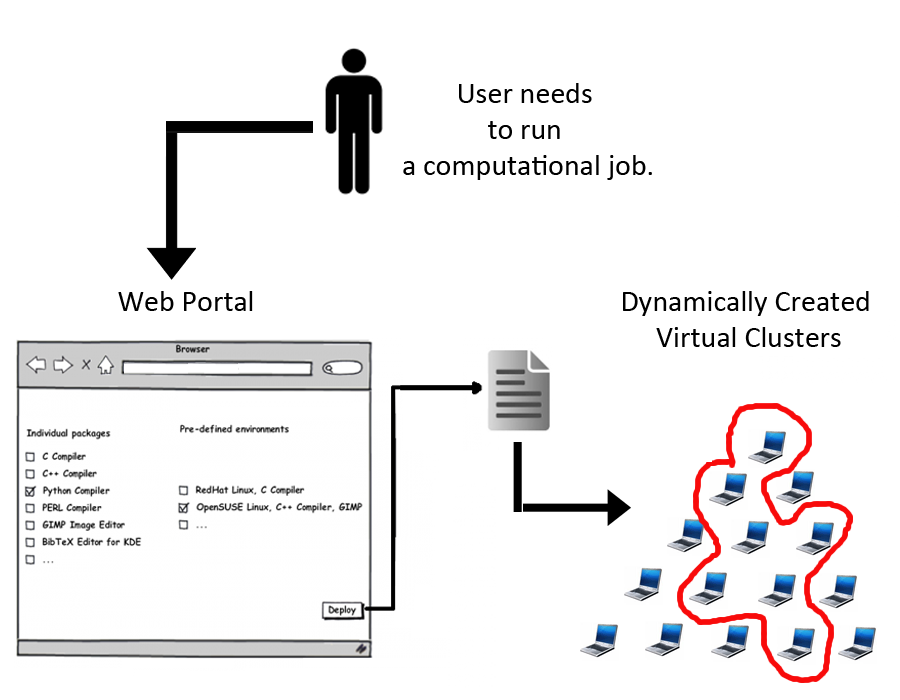
\includegraphics[width=\textwidth]{big_picture}
    \caption{FEUP's Private Cloud Project.}
    \label{fig:big_picture}
  \end{center}
\end{figure}
	
	
\begin{figure}[t]
  \begin{center}
    \leavevmode
    \includegraphics[width=0.5\textwidth]{mockup}
    \caption{Web Portal Interface Mockup.}
    \label{fig:mockup}
  \end{center}
\end{figure}


In order to fully understand what will be developed throughout the next semester, it is needed to comprehend the full scope of the project.
FEUP's private Cloud project is composed by two smaller projects which will be interlinked in the future.
	
Currently, FEUP's computing infrastructures are only accessed by people who have the technical capabilities to interact with the system. These people are the technicians whose area of expertise encompasses outsourcing computing resources to perform computing jobs. If someone from an area that is not Informatics wants to use the system as it is, they need to talk to any of the technicians and waste valuable time (for both parties) cutting through red tape.

As such, this project aims to simplify this whole process and to make FEUP's computing infrastructures more accessible to the academic community, without the users having to spend time studying about the technologies and how the system actually works.

Figure~\ref{fig:big_picture} describes the ``big picture'', the whole computing project being presently worked on at FEUP. As it is possible to see, the system should work in the following manner:


\begin{enumerate}
\item A Chemical Engineering investigator needs to run a job that requires a great deal of computing effort, more than his/her computer can handle;
\item The investigator accesses the portal to be developed and is presented with a layout similar to the one that is shown in Figure~\ref{fig:mockup} where the investigator will be able to either:
	\begin{itemize}
	\item Choose which Linux distribution and which individual packages should be used, as seen on the left side of Figure~\ref{fig:mockup};
	\item Choose a pre-configured environment composed of a pre-selected distribution and already installed packages, as seen on the right side of Figure~\ref{fig:mockup};
	\end{itemize}
\item After choosing either one of the options, the investigator would then press the ``Deploy'' button, which would automatically generate an ISO image containing the information that was passed in the previous step. This ISO image would then be used by the back-end of the project;
\item On the back-end, the ISO image previously deployed would then be used by OpenNebula \footnote{OpenNebula - Virtual Infrastructure Manager that handles the storage, network and virtualization techniques which enable the dynamic placement of interconnected virtual machines on distributed infrastructures.\cite{opennebula}} to dynamically create the virtual cluster where the Chemical Engineering investigator would run his computing job;
\item A \verb,<username:password>, combination would then be returned to the investigator so that he could log into the system and run his computing job in the environment created as he desired.
\end{enumerate}

Through this report, what will be referred as the ``back-end of the project'' consists on the second part of the project (after the ISO image is created), which is currently under development by Nuno Cardoso, a MIEIC - Mestrado Integrado em Engenharia Informática e Computação - student at FEUP, as his Master thesis theme.
	

\section{Motivation and Objectives} \label{sec:goals}

Some computing infra-structures, namely Grids\footnote{Distributed systems that are loosely coupled, heterogeneous and geographically dispersed and act together to perform very large tasks.} and Clusters\footnote{Group of linked computers working closely together as if they were a single machine.}, can be rather inflexible when compared to Clouds, as the latter are supposed to allow the user to take advantage of a myriad of services, and not just computing power.~\cite{brighthub}
	
However, as powerful as these infra-structures can be, they can be deemed useless if people who need to work with them, cannot do it because they have no knowledge of the technologies (one example could be the one used in the previous section, where a Chemical Engineering investigator needed to use the computing system but simply did not have the technical expertise required to interact with the system). As such, this type of issue causes a lack of growth in the use of FEUP's computing system.

This project aims at increasing the usability of the current computing system that exists at FEUP and with this, increase its usage and stop the lack of growth. In order to achieve this goal, a web portal will be developed that will simplify the access to the system. This portal will have a list of software packets and Linux distributions that the user can choose from and create an ISO image which will run the investigator's computing job.

A local software repository will be created and managed, so that the system can still run if there is a network failure and software packets cannot be retrieved from a remote repository. The ISO images will be created and stored in a local server in order to provide reusability, as one ISO image may be used in more than one work session and it would be unnecessary to create the same image again.

A requirements elicitation process will also be held in order to determine what is the best course of action to take when defining and implementing the user interface.

\section{Dissertation Structure} \label{sec:struct}

	Besides the introduction, this document contains three other chapters. In Chapter~\ref{chap:sota}, the current state of the art is described and related work is discussed. In Chapter~\ref{chap:chap3}, the work plan is presented, along with the work methodologies to follow and the task scheduling to be followed next semester during the project development. Finally, in Chapter~\ref{chap:chap4}, a few conclusions regarding the research done are presented.
